 \documentclass{beamer}
\usepackage{listings}
\usepackage{blkarray}
\usepackage{listings}
\usepackage{subcaption}
\usepackage{url}
\usepackage{tikz}
\usepackage{tkz-euclide} % loads  TikZ and tkz-base
%\usetkzobj{all}
\usetikzlibrary{calc,math}
\usepackage{float}
\newcommand\norm[1]{\left\lVert#1\right\rVert}
\renewcommand{\vec}[1]{\mathbf{#1}}
\usepackage[export]{adjustbox}
\usepackage[utf8]{inputenc}
\usepackage{amsmath}
\usepackage{amsfonts}
\usepackage{tikz}
\usepackage{hyperref}
\usepackage{bm}
\hypersetup{
    colorlinks = true,
    linkbordercolor = {white},
    linkcolor={red},
    citecolor={green},
    filecolor={blue},
	menucolor={red},
	runcolor={cyan},
	urlcolor={blue},
	breaklinks=true
}
\usetikzlibrary{automata, positioning}
\usetheme{Boadilla}
\providecommand{\pr}[1]{\ensuremath{\Pr\left(#1\right)}}
\providecommand{\mbf}{\mathbf}
\providecommand{\qfunc}[1]{\ensuremath{Q\left(#1\right)}}
\providecommand{\sbrak}[1]{\ensuremath{{}\left[#1\right]}}
\providecommand{\lsbrak}[1]{\ensuremath{{}\left[#1\right.}}
\providecommand{\rsbrak}[1]{\ensuremath{{}\left.#1\right]}}
\providecommand{\brak}[1]{\ensuremath{\left(#1\right)}}
\providecommand{\lbrak}[1]{\ensuremath{\left(#1\right.}}
\providecommand{\rbrak}[1]{\ensuremath{\left.#1\right)}}
\providecommand{\cbrak}[1]{\ensuremath{\left\{#1\right\}}}
\providecommand{\lcbrak}[1]{\ensuremath{\left\{#1\right.}}
\providecommand{\rcbrak}[1]{\ensuremath{\left.#1\right\}}}
\providecommand{\abs}[1]{\vert#1\vert}

\newcounter{saveenumi}
\newcommand{\seti}{\setcounter{saveenumi}{\value{enumi}}}
\newcommand{\conti}{\setcounter{enumi}{\value{saveenumi}}}
\def\Pr{\mathop{\rm Pr}\nolimits}

\makeatletter
\newenvironment<>{proofs}[1][\proofname]{%
    \par
    \def\insertproofname{#1\@addpunct{.}}%
    \usebeamertemplate{proof begin}#2}
  {\usebeamertemplate{proof end}}
\makeatother

\title{Assignment 3 - (AS3)=UGC / MATH (mathA June 2017), Q.118}
\author{Prashanth Sriram S}
\date{CS20BTECH11039}
\begin{document}

\begin{frame}
\titlepage
\end{frame}

\begin{frame}

\begin{block}{Question}
Suppose the random variable $X$ has the following probability density function
\begin{align}
f(x)=
\begin{cases}
\alpha(x-\mu)^{\alpha-1}e^{-(x-\mu)^\alpha} &x>\mu\\
0 &x\leq\mu,
\end{cases}
\end{align}
Where $\alpha>0, -\infty<\mu<\infty$. Which of the following statements are correct? The Hazard function of $X$ is
\begin{enumerate}
\item A) an increasing function for all $\alpha>0$
\item B) a decreasing function for all $\alpha>0$
\item C) an increasing function for some $\alpha>0$
\item D) a decreasing function for some $\alpha>0$
\end{enumerate}
\end{block}
\end{frame}
\begin{frame}{Required Concepts}
Let $T$ be a non-negative random variable representing the waiting time until the occurrence of an event. For simplicity, we will take the event as death and the waiting time as Survival time.
\begin{block}{Survival Function}
Let us assume that $T$ is a continuous random variable with p.d.f $f(t)$ and c.d.f $F(t)$
\begin{align}
S(t) = \Pr \{T\geq t\} = 1-F(t) = \int_{x}^{\infty}f(x)dx \label{eq:1}
\end{align}

\end{block}
\end{frame}
\begin{frame}{Required Concepts}
\begin{block}{Hazard Function}
Hazard function gives the instantaneous rate of occurrence of the event
\begin{align}
\lambda(t) = \lim_{dt\to0}\frac{\Pr \{t\leq T\leq t+dt|T\geq t \}}{dt} \\
&=\lim_{dt\to0}\frac{\Pr \{t\leq T\leq t+dt \}}{S(t)dt}\\
&=\frac{f(t)}{S(t)}\label{eq:3}
\end{align}
\end{block}
\end{frame}
\begin{frame}{Required Concepts}
\begin{block}{Hazard Function}
From \eqref{eq:1}, 
\begin{align}
\frac{d}{dt}S(t) = -f(t) \label{eq:4}
\end{align}
From \eqref{eq:3} and \eqref{eq:4}
\begin{align}
    \lambda(t) = -\frac{d}{dt}log(S(t))
\end{align}
Integrating on both sides from $0$ to $t$ and using $S(0)=1$,
\begin{align}
-\int_{0}^{t}\lambda(x)dx = log(S(t)) - 0
\end{align}
\end{block}
\end{frame}
\begin{frame}{Required Concepts}
\begin{block}{Hazard Function}
\begin{align}
    S(t) = e^{-\int_{0}^{t}\lambda(x)dx}\label{eq:5}
\end{align}
From \eqref{eq:5} and \eqref{eq:3}, we can find $\lambda(t)$
\end{block}
\end{frame}
\begin{frame}{Solving the question}
\begin{block}{Finding the Survival Function}
\begin{align}
f(x)=
\begin{cases}
\alpha(x-\mu)^{\alpha-1}e^{-(x-\mu)^\alpha} &x>\mu\\
0 &x\leq\mu,\\
\end{cases}\label{eq:8}
\end{align}
\begin{lemma}
\begin{align}
S(x)=
\begin{cases}
e^{-(x-\mu)^\alpha} &x>\mu\\
1 &x\leq\mu
\end{cases} \label{eq:7}
\end{align}
\end{lemma}
\end{block}
\end{frame}
\begin{frame}{Finding Survival function}

\begin{proof}
\begin{align}
\int f(t)dt=\int \alpha(t-\mu)^{\alpha-1}e^{-(t-\mu)^\alpha}dt\\
=-e^{-(t-\mu)^\alpha} + C
\end{align}
If $x>\mu$, 
\begin{align}
S(x) = \int_{x}^{\infty} \alpha(t-\mu)^{\alpha-1}e^{-(t-\mu)^\alpha}dt\\
=-e^{-(t-\mu)^\alpha}]_{x}^{\infty}\\
=e^{-(x-\mu)^{\alpha}} \label{eq:6}
\end{align}
\end{proof}
\end{frame}
\begin{frame}{Finding Survival function}
\begin{proof}
If $x\leq\mu$,
\begin{align}
S(x) = \int_{x}^{\mu}f(t)dt + \int_{\mu}^{\infty}f(t)dt\\
     = 0 + e^{-(\mu-\mu)^{\alpha}}\\
     =1 \label{eq:7}
\end{align}
\end{proof}
From \eqref{eq:5} and \eqref{eq:6}, the lemma is proved
\end{frame}
\begin{frame}{Finding Hazard function}
\begin{block}{Finding $\lambda(x)$}
Using \eqref{eq:6} and \eqref{eq:8}, we get
\begin{align}
\lambda(x) = 
\begin{cases}
\alpha(x-\mu)^{\alpha-1} &x>\mu\\
0 &x\leq\mu \label{eq:5}
\end{cases}
\end{align}
\end{block}
\end{frame}
\begin{frame}{Analysing this function for different values of $\alpha$}
So,\\ if $\alpha>1$, $\lambda(x)$ is an increasing function
\begin{figure}[htp]
    \centering
    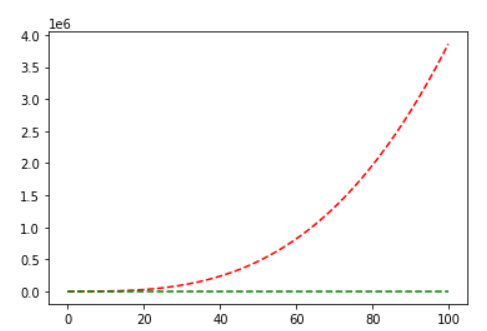
\includegraphics[width=8cm]{alphagrt1.png}
    \caption{$\alpha=2$ for red. $\alpha=1$ for green, $\mu=1$ for both}
    \label{fig:grt1}
\end{figure}
\end{frame}
\begin{frame}{Analysing this function for different values of $\alpha$}
if $0<\alpha<1$, $\lambda(x)$ is a decreasing function
\begin{figure}[htp]
    \centering
    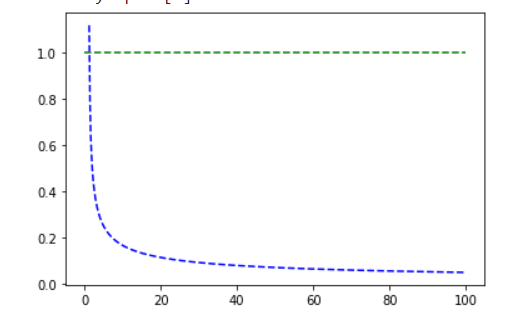
\includegraphics[width=8cm]{alphales1.png}
    \caption{$\alpha=0.5$ for blue. $\alpha=1$ for green, $\mu=1$ for both}
    \label{fig:les1}
\end{figure}
For $\alpha=1$, $\lambda(x)=1$, a constant function.
\end{frame}
\begin{frame}{Conclusion}
So, for some values of $\alpha$, it is an increasing, for some it is a decreasing function\\
Hence, the answer is (C) and (D)
\end{frame}

\end{document}
